\documentclass[10pt,conference]{IEEEtran}
\usepackage[utf8]{inputenc}
\usepackage{amsmath,amssymb}
\usepackage{booktabs}
\usepackage{graphicx}
\usepackage{multirow}
\usepackage{url}
\usepackage[hidelinks]{hyperref}
\usepackage{microtype}
\usepackage{balance}

\begin{document}

\title{The Defect Is in the Arithmetic Between the Files:\\
Static Detection of Exactly-Once Violations in Payment Pipelines}

\author{\IEEEauthorblockN{Abhishek Sharma}
\IEEEauthorblockA{Senior Member, IEEE\\
\texttt{abhicse24@gmail.com} \quad ORCID: 0009-0007-1103-2103}}

\maketitle

\begin{abstract}
Whether a streaming payment pipeline charges a customer twice after a restart
turns on a comparison nobody performs: how long the provider remembers an
idempotency key, against how stale a record can be when the pipeline processes
it for the second time. The first number is in the provider's documentation.
The second is not written anywhere. It is assembled from a checkpoint interval
in one file, a recovery assumption in a runbook, a restart delay in a
third place and a source's lateness bound in a fourth. Each file is defensible
alone, and the fault is in the relation between them. We give a checker that gathers those facts and states the relations, and a
synthesiser that turns each finding into a runnable scenario: these records,
kill the job here, bring it back after this long, and the provider will show
two charges for one order.

The central measurement is how far apart the evidence lies. Across a corpus of
630 pipelines we generated, 210 of 515 findings cannot be derived from fewer
than three artifacts, and no single artifact yields more than 35 of the 305
duration findings. Executing the witnesses corrected our own rules: two were
demoted after their scenarios produced a repeated call that the provider's
idempotency absorbed rather than a second charge. All 16 selected live
witnesses reproduced their predicted observable against a real Kafka broker
with a real process kill, and a matched control in which the provider never
forgets the key did not, which is what makes the second charge attributable to
the key lifetime and not to the replay.

Fault injection finds the same defects only if the tester already assumed a
long enough outage: one willing to simulate five minutes finds 15\% of them,
and 12 hours is needed for all. A configuration sweep also locates a
configuration with no application-level fix, where above roughly a 14-minute
recovery assumption the transaction timeout required to survive it exceeds the
broker's own cap. That threshold holds under the broker's default 15-minute
cap and a modelled drain rate of one, and the sweep locates a threshold rather
than estimating how common it is in deployed pipelines.
\end{abstract}

\begin{IEEEkeywords}
static analysis, stream processing, exactly-once semantics, idempotency,
payment systems, Apache Kafka
\end{IEEEkeywords}

\section{Introduction}

A payment pipeline reads orders, calls a provider to move money, and writes to
a ledger. It is configured for exactly-once: a transactional sink, a
deduplicating operator, an idempotency key on every call. Then the job dies at
lunchtime, somebody notices at two, and when it comes back it reprocesses
everything since its last checkpoint. Some of those customers are charged
twice.

Nothing in the pipeline is obviously wrong. The key is derived from the order
id, so the retry is recognisable. The provider does deduplicate. The sink is
transactional. What went wrong is that the provider stopped remembering the key
some hours before the replay arrived, and the replay was therefore a new
request as far as it was concerned.

That defect is a comparison between two numbers. One is in the provider's API
documentation. The other does not exist in any file: it is the longest a record
can go between its first processing and its second, and computing it needs a
checkpoint interval from the engine config, an assumption about how long a job
may stay dead from a runbook, a restart delay from a third place, and a
source's lateness bound from a fourth. No reviewer holds four artifacts at
once. No linter reads the provider's documentation. The pipeline passes every
review it will ever get.

This paper is about finding those before the outage. The contribution is in
three parts.

A **model that spans artifacts.** Facts are gathered from the engine
configuration, the client properties, the job SQL, the runbook and a
declaration of what the provider guarantees, and each fact keeps a record of
where it came from. From them we derive the \emph{replay horizon}, and state
the defect classes as relations against it. Thirteen checks, split between
structural defects a careful reviewer could find and duration defects that
require the arithmetic.

**Witnesses.** A static finding about a payment pipeline is easy to dismiss, so
each becomes a runnable scenario with a predicted observable. Running them
against a real Kafka broker, with the pipeline process really killed and a
provider that really forgets, either produces the second charge or does not.
Every run is paired with a control in which the provider never forgets, so the
second charge is attributable to the key lifetime rather than to the replay.

**An evaluation that corrected the thing being evaluated.** Two of our rules
predicted a double charge and were wrong: their witnesses reproduce a repeated
call that the provider absorbs. Both were demoted to medium severity and their
witnesses now predict two invocations and one charge. The corpus's own clean
baseline turned out to be defective under a rule added later, which is reported
rather than quietly fixed.

One finding has no fix at the pipeline level. Kafka caps a producer's requested
transaction timeout at fifteen minutes by default, and surviving a recovery
assumption longer than about fourteen minutes requires more than that. The
choice is then between a shorter assumption, a cluster-wide broker change, and giving up the transactional sink. None of the three is a setting in the
job.

\section{Background and related work}

\subsection{Exactly-once in stream processors}

Flink's checkpointing and Kafka's transactional producer give end-to-end
exactly-once for effects inside the system's own boundary: a record consumed,
transformed and written back to Kafka can be made to appear once. The
literature and documentation on this is mature, and we assume rather than
restate it.

An external payment call is outside that boundary. The money moves before the
checkpoint completes, no two-phase commit can take it back, and the only
defence is the provider's idempotency. Everything in this paper is about that
gap, which is where payment pipelines actually live.

\subsection{Fault recovery and stream benchmarking}

Vogel et al.~\cite{vogel2024} benchmark fault recovery across stream processing
frameworks, measuring recovery time and throughput after failure. That is the
behaviour our duration checks depend on, measured empirically; what it does not
do, and does not set out to do, is decide whether a given configuration is
correct. Mohammad~\cite{mohammad2025} surveys Kafka design patterns and
benchmarking practice across 42 studies, finding recurring architectural
patterns; again a description of what people build rather than a check on it.

\subsection{Idempotency as a contract}

Idempotency keys are ubiquitous in payment APIs and the mechanism is well
understood: the client supplies a key, the provider remembers it, and a repeat
within its memory is a no-op returning the original result. What is less often
stated is that the memory is finite, that its length is part of the API
contract, and that a client whose retries can outlive it has no idempotency at
all. Practitioner writing does say so. The advice to never expire a key before the
client's longest retry window is common, and it is treated as a guideline
instead of something to check. The formal treatment
in~\cite{t8} gives operation identity and a conformance suite for the
provider's side; what is missing on the consumer's side is the arithmetic
relating that lifetime to how long a replay can take, which is what this paper
supplies.

\subsection{Static analysis and witnesses}

Reporting a defect together with evidence that it is real is an old idea in
verification. SV-COMP's witness formats let one tool's verdict be validated by
another, and the correctness-witness line of work exists precisely because a
verdict without a checkable artifact asks to be taken on trust. Our witnesses
are of the violation kind and are validated by execution rather than by a
second analyser, which suits a defect whose observable, money moved twice, is unambiguous.

What we did not find, and searched for, is a static checker for the
configuration relations below. Practitioner writing states several of them as
advice: keep the transaction timeout above the checkpoint interval plus
expected downtime; never expire an idempotency key before the client's longest
retry window. The advice is correct and nothing checks it.

\subsection{Sibling work}

ReconStream~\cite{reconstream} gives a temporal correctness contract for
streaming reconciliation, in which a verdict is admissible only once a
source's declared lateness bound has passed. Its notion of a declared bound is
what the replay horizon here borrows for its source term, and the reconciliation
shape in our corpus is its setting. The two papers share a shape of argument, a correctness property that relates
durations instead of states, applied at different points of the pipeline. Operation identity, what
makes two records the same money movement, follows~\cite{t8}; the failure
patterns the checks encode draw on~\cite{t4}.

\section{The replay horizon}

Write $\mathrm{cp}$ for the checkpoint interval, $\mathrm{pause}$ for the
minimum pause between checkpoints, $\mathrm{down}$ for the longest a job is
assumed to stay dead, $\mathrm{restart}$ for the restart delay, and
$\Lambda_s$ for the declared lateness bound of source $s$. On recovery the job
resumes from its last checkpoint, so everything processed since is replayed;
while it was down the input accumulated, and draining that backlog takes time
proportional to the outage. Records still in flight when the job died arrive
within their source's bound. Putting those together,
\begin{equation}
H = \mathrm{cp} + \mathrm{pause} + \mathrm{down} + \mathrm{restart}
    + \delta(\mathrm{down} + \mathrm{restart}) + \max_s \Lambda_s ,
\label{eq:horizon}
\end{equation}
where $\delta$ is the drain factor, one by default. $H$ is the age a record can
have reached when it is processed for the second time.

Two of the six terms come from the engine's configuration, one from a runbook,
one from a job definition, and $\delta$ is an operational estimate. That
spread is the reason $H$ is not computed anywhere, and computing it is most of
what the checker does.

\subsection{Two families of defect}

\textbf{Structural} defects are about shape: an effect that no commit protocol
covers, a key built from a fresh UUID, a consumer reading uncommitted output of
a transactional producer, an effect placed upstream of the deduplication meant
to guard it. A careful reviewer reading the job can find these.

\textbf{Duration} defects are relations against $H$. The provider forgets the
idempotency key before the replay arrives ($\mathrm{ttl} < H$); the dedup
state expires before the duplicate it exists to catch ($\mathrm{state\ ttl} <
H$); the broker aborts the transaction before the job returns; the client's own
retry window outlives the key. These are the ones that survive review, and they
are arithmetic.

Table~\ref{tab:rules} lists the thirteen checks. Each is a sufficient condition
for a violation, not a certificate of correctness. A pipeline with no findings has not been
proved exactly-once, and we are careful not to say otherwise.

\begin{table}[t]
\caption{The checks. ``Artifacts'' is how many separate files the finding's
evidence spans.}
\label{tab:rules}
\centering
\footnotesize
\begin{tabular}{llr}
\toprule
& & artifacts \\
\midrule
\multicolumn{3}{l}{\emph{structural}} \\
SC001 & effect outside the commit protocol & 1 \\
SC002 & non-deterministic idempotency key & 1 \\
SC003 & missing idempotency key & 1 \\
SC004 & uncommitted read of transactional output & 1 \\
SC005 & shared transactional id prefix & 2 \\
SC006 & effect upstream of deduplication & 1 \\
SC007 & non-idempotent sink under at-least-once & 1 \\
\midrule
\multicolumn{3}{l}{\emph{duration}} \\
SC100 & undeclared provider key lifetime & 3 \\
SC101 & key lifetime below the replay horizon & 3 \\
SC102 & dedup state TTL below the replay horizon & 3 \\
SC103 & transaction timeout below the downtime & 3 \\
SC104 & delivery timeout above transaction timeout & 1 \\
SC105 & client retry window above key lifetime & 1 \\
SC106 & required transaction timeout exceeds the broker cap & 2 \\
\bottomrule
\end{tabular}
\end{table}

\subsection{Reading the facts out of the files}

Four front-ends, one per place a fact lives. \texttt{flink-conf.yaml} gives the
checkpoint interval, the restart delay and the state TTL. The Kafka client
properties give the transaction and delivery timeouts and the consumer's
isolation level. The job SQL gives the topology: which tables are read, which are written,
whether a \texttt{ROW\_NUMBER} deduplication is present. The connector options
give the delivery guarantee and any watermark lateness. A
runbook gives the recovery assumption, if one is written down.

The fourth is different. How long the provider remembers an idempotency key is
a fact about the provider: it is in their API reference, it is load-bearing for
correctness, and no artifact in the repository records it. We ask for it in a
small manifest, in the sense of~\cite{t8}'s provider-aware contract, and when
it is absent the checker emits a finding (SC100) rather than assuming a value.
Guessing would mean asserting something about a third party on no basis, and
the assumption would then be invisible in exactly the way the rest of the paper
is complaining about.

The SQL reader is deliberately shallow: it recognises the shapes these
pipelines are written in and reports what it cannot place, so a fact it fails
to find becomes a statement about incomplete evidence rather than a silent
default. Each extracted fact carries its origin, which is what lets a finding cite the files it depends on, and what makes the
measurement in Section~\ref{sec:artifacts} possible.

\subsection{A worked example}

The artifacts in the repository's \texttt{data/example-pipeline} are ordinary.
The engine checkpoints every 60 seconds and restarts after 30. The producer
sets \texttt{transaction.timeout.ms=900000}, which is Kafka's default. The
runbook records a 45-minute worst observed recovery, with a note about a
weekend page that went unanswered for 40 minutes. The provider documents a
24-hour idempotency key. Each number is defensible and none would be questioned
in review.

Equation~\eqref{eq:horizon} gives $H = 1.54$ hours, comfortably inside the
24-hour key. The transaction timeout is not: surviving a checkpoint plus 45
minutes of downtime plus the restart needs 46.5 minutes, and 15 minutes is
configured. Raising it does not help, which is the next section.

\section{The defect with no fix}

Kafka caps a producer's requested transaction timeout at
\texttt{transaction.max.timeout.ms}. We read the value from a running broker rather than from documentation:
apache/kafka 3.9.0 reports 900{,}000\,ms, and its synonym chain marks it
\texttt{DEFAULT\_CONFIG}. The refusal is measured too, at the boundary. A Java
producer calling \texttt{initTransactions()} against that broker is granted
60{,}000\,ms and granted 900{,}000\,ms, and refused at 900{,}001\,ms with
\emph{the transaction timeout is larger than the maximum value allowed by the
broker}. One millisecond either side of the cap is the difference between a
pipeline that starts and one that does not.

So for an exactly-once pipeline, the requirement $\mathrm{cp} + \mathrm{down} +
\mathrm{restart} \le \text{cap}$ bounds the recovery assumption rather than the
configuration. With 60-second checkpointing and a 30-second restart delay, any assumption
above 13.8 minutes is unsatisfiable; the bound moves between 9.8 and 14.7
minutes across the checkpoint intervals we swept. Every one of those figures
is conditional on four things we chose or measured: the broker's default cap
of 900{,}000\,ms, the drain factor of one held throughout, the replay-horizon
formula of~\eqref{eq:horizon}, and the recovery model in which a job is
restarted after a bounded outage. A cluster with a raised cap has no such
threshold, and a drain factor above one lowers it.

This is not a misconfiguration. It is a configuration that does not exist, and the remedies (shorten the recovery assumption, raise the cap cluster-wide,
or drop the transactional sink) are all decisions above the pipeline. We
report it as a distinct rule (SC106) from the ordinary too-small timeout
(SC103), because telling a team to raise a number they cannot raise is worse
than telling them nothing.

\section{Witnesses}

A finding becomes a scenario: the input records, a fault schedule, and a
predicted observable. For a key-lifetime defect the scenario is one order,
a failure after the charge and before the checkpoint, and an outage long enough
for the key to expire; the prediction is two charges where there should be one.

\textbf{Witnesses run compressed.} A replay horizon of hours cannot be waited
out once per finding, let alone hundreds of times. Every duration check is an
inequality between durations and nothing else, so multiplying every duration in
a witness by one positive factor leaves each comparison, and therefore the
defect, unchanged. Witnesses are synthesised in the pipeline's units and
executed at a fraction of them. That is an argument about our own method, so we
measure it: Section~\ref{sec:results} reports the verdict of every witness
across four orders of magnitude of compression.

\paragraph{One witness, end to end} The boundary case whose key lifetime sits
one second under the replay horizon produces this. Compressed so the lifetime
is 30 seconds, the witness says: one order, fail once the charge has gone
through, stay down for 30.0 seconds. The pipeline's own log, from the run and
from the sufficient-lifetime control, differs in one line:

\begin{center}
\footnotesize
\begin{tabular}{@{}l@{}}
\texttt{start pid=34847 restored=0 keys} \\
\texttt{effect ord-witness-1 key=ord-witness-1:stable charged=True} \\
\texttt{start pid=35991 restored=0 keys} \\
\texttt{effect ord-witness-1 key=ord-witness-1:stable \textbf{charged=True}} \\
\midrule
\texttt{...control, lifetime long enough to cover the replay:} \\
\texttt{effect ord-witness-1 key=ord-witness-1:stable \textbf{charged=False}} \\
\end{tabular}
\end{center}

The key is identical in both. The record is identical. The kill is identical.
On the tightest of the six runs that cleared the scaled 30-second lifetime, the
provider observed 30.6 seconds between the two attempts, six tenths of a
second of margin, and in one case that was inside the lifetime and in the
other it was not. Nothing about the
pipeline distinguishes the two runs, which is the argument for why the defect
is in the configuration rather than in the code.

\textbf{Some findings get no witness.} A shared transactional id prefix needs a
second job to manifest; an undeclared key lifetime is the absence of a fact
rather than a fact. Saying a rule has no runnable scenario is better than
shipping one that demonstrates nothing, and the coverage figure in
Section~\ref{sec:results} counts the gap honestly.

\section{Corpus and setup}

Five pipeline shapes, drawn from things payments teams build: taking a capture
to a processor, issuing a refund, reconciling a ledger against a bank feed,
paying out a batch, retrying a failed charge. Twenty-one mutations, each
introducing exactly one defect, crossed with the shapes, twice per combination,
over three seeds: 630 pipelines, of which 150 are negatives.

The mutations named after the rule meant to catch them are the weakest part of
the corpus and we treat them as such. The same author wrote the mutation and
the check, so a high score there measures implementation correctness rather
than detection power. The cases that carry evidential weight are the other two
kinds. Four \emph{boundary} mutations put a lifetime one second either side of
the replay horizon, so distinguishing them requires computing $H$ correctly
from all six terms; a checker that recognised mutation names rather than doing
arithmetic would fail them whichever way it erred. Two \emph{decoys} look
alarming and are correct: two-second checkpointing, which shortens the horizon
and makes every relation easier to satisfy, and a long client retry window that
still fits inside the key's lifetime.

\begin{table}[t]
\caption{The corpus. Sixteen mutations name the rule meant to catch them and
are the weakest evidence; the boundary and decoy cases are the informative
ones.}
\label{tab:corpus}
\centering
\footnotesize
\begin{tabular}{llr}
\toprule
kind & correct answer & cases \\
\midrule
16 defect mutations       & the named rule & 480 \\
clean pipelines           & no finding     &  30 \\
boundary, defective side  & SC101 or SC102 &  60 \\
boundary, correct side    & no finding     &  60 \\
2 decoys                  & no finding     &  60 \\
\midrule
\multicolumn{2}{l}{5 shapes $\times$ 21 mutations $\times$ 2 $\times$ 3 seeds} & 630 \\
\bottomrule
\end{tabular}
\end{table}

The five shapes are a capture taken to a processor, a refund, a reconciliation
of a ledger against a bank feed, a batch payout, and a dunning retry. The
reconciliation shape is P5's setting and carries its source lateness bound,
which is why its replay horizon exceeds what the engine configuration alone
would suggest. It is the one place in the corpus where a fact from a job
definition changes a duration relation.

Execution uses apache/kafka 3.9.0 in KRaft mode, a pipeline process killed with
SIGKILL, and an HTTP provider that expires keys on a timer. Nothing about the
recovery is modelled: what is replayed is whatever the broker redelivers from
the last committed offset.

\section{Results}
\label{sec:results}

\subsection{Detection}

Over 630 pipelines the checker recovers every injected defect and reports
nothing on any of the 150 negatives, at 3.8 microseconds per pipeline. The
recall figure should be read narrowly for the reason given above. The boundary
cases are the informative part: all 30 instances either side of each threshold
are classified correctly, on a two-second difference in configuration.

\begin{table}[t]
\caption{Detection over 630 pipelines. The boundary and decoy rows are the
informative ones; the mutation rows are matched to their rules by construction.}
\label{tab:detection}
\centering
\footnotesize
\begin{tabular}{lrrr}
\toprule
case kind & cases & correct & findings raised \\
\midrule
injected defects (16 mutations) & 480 & 480 & as expected \\
clean pipelines                 &  30 &  30 & none \\
boundary, defective side        &  60 &  60 & the expected rule \\
boundary, correct side          &  60 &  60 & none \\
decoys (look wrong, are right)  &  60 &  60 & none \\
\midrule
total                           & 630 & 630 & 0 false positives \\
\bottomrule
\end{tabular}
\end{table}

\subsection{How many files a finding needs}
\label{sec:artifacts}

\begin{figure}[t]
\centering
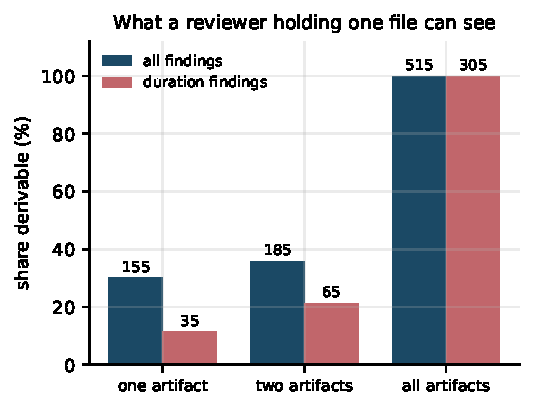
\includegraphics[width=0.85\columnwidth]{../figures/fig1_artifacts.pdf}
\caption{Findings derivable from a restricted view of the artifacts.}
\label{fig:artifacts}
\end{figure}

Of 515 findings across the corpus, 245 are derivable from a single artifact, 60
need two, and 210 need three. Restricting to the 305 duration findings sharpens
it: 210 need three artifacts, 30 need two, and 65 need one.

Figure~\ref{fig:artifacts} puts that in the reviewer's position. The most
informative single artifact yields 155 of 515 findings, and only 35 of the 305 duration findings, 11.5\% of them. The best pair reaches 185 findings and 65
duration findings. A reviewer reading the job, or the job and the producer
properties, sees the structural defects and almost none of the arithmetic.

\begin{table}[t]
\caption{Findings derivable from a restricted view. ``Duration'' is the subset
that is arithmetic against the replay horizon.}
\label{tab:artifacts}
\centering
\footnotesize
\begin{tabular}{lrrrr}
\toprule
view & findings & share & duration & share \\
\midrule
best single artifact & 155 & 30.1\% & 35 & 11.5\% \\
best pair            & 185 & 35.9\% & 65 & 21.3\% \\
best triple          & 245 & 47.6\% & --- & --- \\
everything           & 515 & 100\%  & 305 & 100\% \\
\bottomrule
\end{tabular}
\end{table}

This is the paper's central measurement, and it is what the introduction's
claim rests on: these defects survive review because review is conducted one
file at a time.

\subsection{Do the witnesses reproduce?}

\begin{figure}[t]
\centering
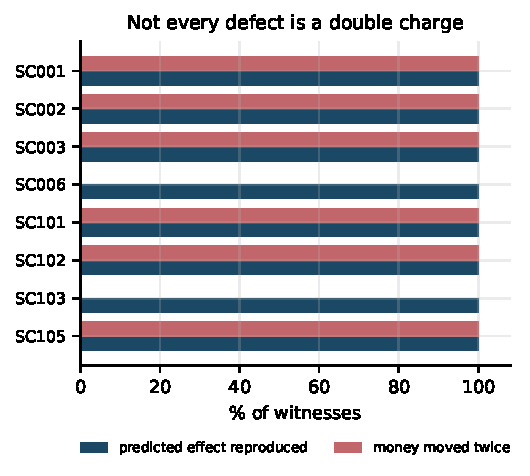
\includegraphics[width=0.85\columnwidth]{../figures/fig4_witness.pdf}
\caption{Witness outcomes by rule. Reproducing the predicted effect and moving
money twice are different things.}
\label{fig:witness}
\end{figure}

Of 515 findings, 335 admit a witness (65\%; 70.5\% of the duration findings).
Every one of the 335 reproduces its predicted observable. Only 245 of them, 73\%, move money twice.

That gap is a correction to our own rules rather than a property of the
pipelines. Two rules originally predicted a double charge: an effect placed
upstream of its deduplication, and a transaction timeout too short to survive
the downtime. Both produce a second call to the provider, and with a sound key
still in its lifetime the provider absorbs it. The pipelines are wrong: they have no defence of their own and are correct
only because the provider is. But they are not double-charging, and reporting
them as though they were would have been a false alarm on every one. Both were demoted to medium severity and
their witnesses now predict two invocations and one charge.

\begin{table}[t]
\caption{Witness outcomes by rule. ``Reproduced'' is the predicted observable;
``charged twice'' is money actually moving a second time. Rules with no
witness describe conditions a single-record scenario cannot exhibit.}
\label{tab:witness}
\centering
\footnotesize
\begin{tabular}{lrrrr}
\toprule
rule & findings & witnessed & reproduced & charged twice \\
\midrule
SC001 & 30 & 30 & 100\% & 100\% \\
SC002 & 30 & 30 & 100\% & 100\% \\
SC003 & 30 & 30 & 100\% & 100\% \\
SC004 & 30 & --- & --- & --- \\
SC005 & 30 & --- & --- & --- \\
SC006 & 30 & 30 & 100\% & 0\% \\
SC007 & 30 & --- & --- & --- \\
SC100 & 30 & --- & --- & --- \\
SC101 & 60 & 60 & 100\% & 100\% \\
SC102 & 60 & 60 & 100\% & 100\% \\
SC103 & 60 & 60 & 100\% & 0\% \\
SC104 & 30 & --- & --- & --- \\
SC105 & 35 & 35 & 100\% & 100\% \\
SC106 & 30 & --- & --- & --- \\
\bottomrule
\end{tabular}
\end{table}

Six rules are sufficient on their own for a double charge: the three key
defects and the three lifetime defects. Table~\ref{tab:witness} and
Figure~\ref{fig:witness} separate them.

Compression does not change any verdict. All 114 witnesses give identical
results across factors spanning four orders of magnitude, which is what the
homogeneity argument predicts and is worth having measured rather than assumed.

\subsection{Against a real broker}
\label{sec:live}

Sixteen witnesses were replayed against apache/kafka 3.9.0, each in three
arms: as synthesised, with a provider that never forgets the key, and with a
provider whose key lifetime is finite but comfortably longer than the replay
takes. Forty-eight executions, no errors. All 16 selected live witnesses
reproduced their predicted observable.

What that arm does and does not exercise is worth stating plainly, because
``on a real broker'' can be read for more than it is. It uses a real Kafka
broker, a real process death by \texttt{SIGKILL}, a real consumer group
eviction and an HTTP provider with a real key lifetime. It does not use Flink:
there is no Flink checkpointing, no rescaling, and no transactional Flink sink
in this arm. The worker is a purpose-built consumer that commits offsets and
calls the provider, which is the smallest thing that can exhibit the
observable, and the sixteen witnesses are selected from the corpus rather than
being all of it. The claim is therefore about the predicted observables of
those sixteen, not about Flink's behaviour under recovery.

\begin{table}[t]
\caption{Live execution. ``inf'' is the control whose provider never forgets;
``suf'' is the control with a finite but sufficient lifetime. The gap is
between the two attempts, on the provider's clock, against a 30-second scaled
key lifetime.}
\label{tab:live}
\centering
\footnotesize
\begin{tabular}{llrrrr}
\toprule
rule & & gap (s) & def. & inf & suf \\
\midrule
SC101 & key lifetime below horizon & 30.6--48.0 & 2 & 1 & 1 \\
SC102 & state TTL below horizon    & 30.6--32.5 & 2 & 1 & 1 \\
SC105 & retry window above lifetime& 30.8--48.0 & 2 & 1 & 1 \\
\midrule
SC001 & effect not idempotent      & 6.0 & 2 & 2 & 2 \\
SC002 & non-deterministic key      & 5.9 & 2 & 2 & 2 \\
SC003 & missing key                & 5.9 & 2 & 2 & 2 \\
\midrule
SC006 & effect before dedup        & 0.0 & 1 & 1 & 1 \\
SC103 & transaction timeout        & 5.9--6.0 & 1 & 1 & 1 \\
\bottomrule
\end{tabular}
\end{table}

Table~\ref{tab:live} separates three behaviours, and the separation is the
result. The three lifetime defects charge twice as configured, once when the
provider never forgets, and once again when it forgets only after a lifetime
long enough to cover the replay. The observed gap exceeds the key lifetime in
exactly those six runs and in no other. That is the mechanism the rules claim,
observed rather than argued.

The three key defects charge twice in all three arms. This is correct and
worth stating: when the key is absent, or freshly generated on each attempt,
no lifetime helps, because the provider has nothing to recognise. Their second
charge is attributable to the key rather than to the lifetime, and the
experiment says so by the controls failing to remove it.

SC006 and SC103 charge once everywhere, agreeing with the interpreter.

\paragraph{An earlier version of this experiment was measuring the harness}
Witnesses are executed compressed, and the first live arm scaled key lifetimes
to 1.2 seconds. Killing the worker, waiting for the consumer group to evict it
and restarting costs about six seconds of real time, measured at 5.9 to 6.0
seconds across repetitions, so every key expired during the restart whatever
downtime the witness specified. Under that arrangement SC103
witnesses whose configured downtime was nineteen milliseconds reproduced a
double charge, which is not a result about SC103 but a result about our test
rig.

The tell was in the results table: a column showing the configured downtime
sitting three orders of magnitude below the lifetime it was supposed to
outlast. The fix has three parts, and all three are needed. Scale lifetimes to
thirty seconds, several times the overhead. Record the gap the provider
actually observed, so the comparison against the lifetime can be checked rather
than assumed. And add the sufficient-lifetime arm: if the rig were expiring
keys on its own, that arm would charge twice as well, and it charges once in
every one of the runs where it should.

We report this at length because the failure was silent in the direction that
flatters the paper. A harness that expires keys on its own confirms every
lifetime defect put to it.

\subsection{What testing would cost}

\begin{figure}[t]
\centering
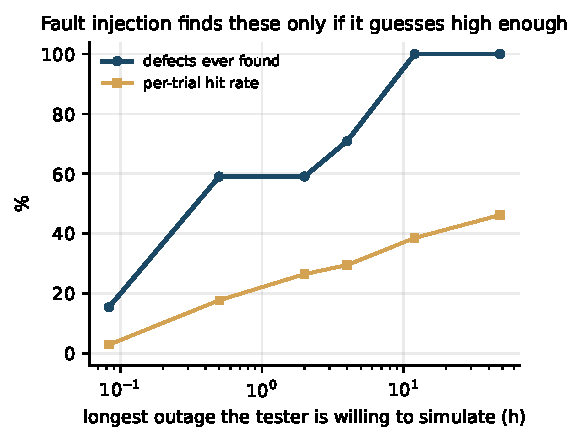
\includegraphics[width=0.85\columnwidth]{../figures/fig2_testing.pdf}
\caption{A fault-injection tester finds these only if its assumed worst outage
is long enough. No number of trials substitutes for guessing high.}
\label{fig:testing}
\end{figure}

The alternative to reading the configuration is injecting faults and watching
for a double charge. It works, and Figure~\ref{fig:testing} shows what it
depends on. Our tester is given every advantage: it knows to kill the job, it
kills at the worst moment rather than a random one, and it inspects the
provider directly instead of waiting for a complaint. The only thing drawn at
random is how long the job stays down.

A tester whose longest simulated outage is five minutes finds 15\% of the
duration defects, and more trials do not help. The trigger is outside the distribution it
samples from. At thirty minutes it reaches 59\%, at four hours
71\%, and only at twelve hours does it find all of them. The per-trial hit rate
never exceeds 46\% even when the ceiling is two days.

\begin{table}[t]
\caption{Duration defects found by a fault-injection tester, as a function of
the longest outage it is willing to simulate.}
\label{tab:testing}
\centering
\footnotesize
\begin{tabular}{rrr}
\toprule
longest simulated outage & defects ever found & per-trial hit rate \\
\midrule
5 min  &  15\% &  2.9\% \\
30 min &  59\% & 17.8\% \\
2 h    &  59\% & 26.5\% \\
4 h    &  71\% & 29.5\% \\
12 h   & 100\% & 38.6\% \\
48 h   & 100\% & 46.2\% \\
\bottomrule
\end{tabular}
\end{table}

This is the honest form of the argument for static analysis here. It is not
that testing cannot find these defects. It is that testing finds them only if someone already suspected that the outage could be long enough, which
is the fact the checker computes, in 3.8 microseconds, from files the team already
has.

\subsection{How much of the configuration space is affected}

\begin{figure}[t]
\centering
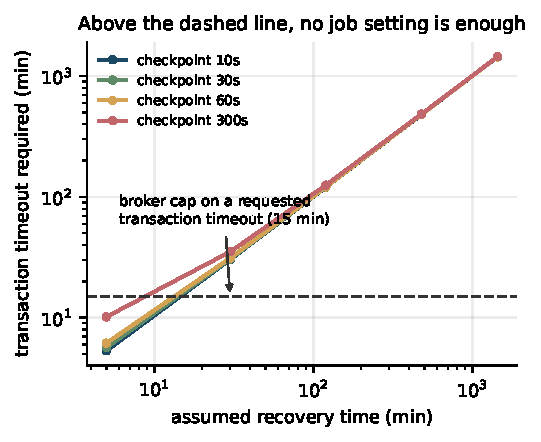
\includegraphics[width=0.85\columnwidth]{../figures/fig3_broker_cap.pdf}
\caption{Required transaction timeout against the assumed recovery time. The
dashed line is the broker's cap on what a producer may request.}
\label{fig:cap}
\end{figure}

Sweeping 960 combinations of checkpoint interval, recovery assumption, key lifetime, state TTL and transaction timeout, each drawn from values
practitioners use, 86.7\% produce at least one finding. That number is a
property of our menus and not of the field, and we do not present it as
prevalence. What transfers is the threshold in Figure~\ref{fig:cap}: the
required transaction timeout grows with the recovery assumption and crosses the
broker's cap at a recovery assumption of about fourteen minutes, after which no
configuration of the job is sufficient.

\section{Discussion}

\paragraph{The unit of review is wrong} Every artifact in the worked example
passes review. The pipeline does not. Code review, linting and configuration
validation are all organised around one file at a time, and the defects that
matter most here are precisely those that no file contains. A checker that
spans artifacts is a small thing technically and a different thing
organisationally.

\paragraph{One fact has no home} The provider's key lifetime is load-bearing
for correctness and lives in no repository. We ask for it to be declared, in
the sense of~\cite{t8}'s provider-aware contract, and treat its absence as a
finding rather than defaulting it. A tool that guessed would be asserting
something about a third party it has no basis for.

\paragraph{The horizon is an operational number, not an engineering one}
Four of the six terms in~\eqref{eq:horizon} come from configuration. The one
that dominates is not: how long a job may stay dead is a property of who is on
call, how alerts are routed, and whether the page goes out at three in the
afternoon or three in the morning. Shortening it is the cheapest fix for every
duration defect here, and it is the one no code change achieves. The tool's
most useful output may be that a number in a runbook is load-bearing for
correctness, which is not where teams look for correctness arguments.

\paragraph{Execution as a check on the checker} The most useful thing the
witnesses did was disagree with us. Two rules were wrong about their own
severity, and no amount of re-reading them would have shown it; running them
did, in seconds. We would recommend the arrangement to anyone writing a
checker whose findings have an observable consequence.

\section{Limitations}

The corpus is generated by us, and the mutations named after rules are matched
to those rules by construction. The boundary cases, the decoys and the live
execution are the parts that carry evidence; the headline recall number is not.

The execution arm is not Flink. Expressing an external HTTP effect in Flink SQL
requires a custom connector, and writing one would have put more of our own
code between the witness and the result. The replay semantics exercised are
Kafka's real offset commit and redelivery, and the process really dies, but
operator-level checkpointing and rescaling are not exercised. Pipelines are
single-partition throughout.

Both halves of the broker cap are now measured on one broker: its configured
value, and its refusal at one millisecond past that value. Neither is a
survey. A cluster whose operator has raised
\texttt{transaction.max.timeout.ms} has a different cap and a different
threshold, and we tested the default on apache/kafka 3.9.0 rather than a
distribution of deployed settings.

Each check is sufficient for a violation, not necessary. A pipeline with no
findings has not been proved correct, and the checker says so.

The live arm covers sixteen witnesses, two per rule that admits one, rather
than the whole corpus: three arms at roughly a minute each puts an exhaustive
run beyond a reasonable budget. The interpreter covers every witness and agrees
with the broker on all sixteen, which is some comfort and not a substitute.

The drain factor, how long a backlog takes to clear relative to the outage
that produced it, is held at one throughout and never swept. A busier
pipeline drains more slowly and has a longer horizon than we compute, so our
estimate is optimistic in a direction that matters.

The configuration sweep uses menus we assembled from values practitioners
report. It supports a statement about where the threshold lies, not about how
common the defect is in deployed systems, and we have no field data.

\section{Conclusion}

The question of whether a restart charges a customer twice has an answer, and
the answer is arithmetic between numbers that live in four different files and
one external document. Gathering them takes microseconds and finding the
defects takes a comparison; what makes them survive is that nothing gathers
them. Two things surprised us in the building. Executing the witnesses demoted
two of our own rules, because a duplicate call the provider absorbs is not a
double charge. And one configuration turns out to have no fix at the pipeline level at all:
past a fourteen-minute recovery assumption, under the broker's default cap and
a modelled drain rate of one, the transaction timeout that would be needed is
larger than the broker will grant. The sweep locates that threshold; it does
not say how many deployed pipelines sit past it, and we make no estimate of
prevalence.

\section*{Artifact availability}

Code, corpus generator, Docker configuration and every results file are at
\url{https://github.com/abhisheksharma2411/streamcheck}. An archival DOI is forthcoming. \texttt{make reproduce} runs the pipeline
from a clean checkout: it starts a Kafka broker, runs every experiment,
regenerates each figure from the raw results and rebuilds this paper. No number
in the text is entered by hand; \texttt{scripts/verify\_claims.py} checks each
one against the results files.

\begin{thebibliography}{99}

\bibitem{vogel2024}
A.~Vogel, S.~Henning, E.~Perez-Wohlfeil, O.~Ertl, and R.~Rabiser,
``A comprehensive benchmarking analysis of fault recovery in stream processing
frameworks,'' in \emph{Proc. 18th ACM Int. Conf. Distributed and Event-Based
Systems (DEBS)}, 2024. doi:10.1145/3629104.3666040.

\bibitem{mohammad2025}
M.~Mohammad, ``Analysis of design patterns and benchmark practices in Apache
Kafka event-streaming systems,'' arXiv:2512.16146, Dec.~2025.

\bibitem{reconstream}
A.~Sharma, ``When is a reconciliation break real? A temporal correctness
contract for streaming financial reconciliation,'' manuscript in preparation,
2026.

\bibitem{t8}
A.~Sharma, ``A provider-aware formal contract and conformance suite for payment
idempotency,'' under review, 2026.

\bibitem{t4}
A.~Sharma, ``Large language models generate retry-safe payment services,''
under review, 2026.

\end{thebibliography}

\balance
\end{document}
